Computer security is a broad, interdisciplinary field with technical and non-technical challenges.
An important subset of the technical aspects can be modeled and studied mathematically~\cite{piessens2024}.
At its core, computer security is concerned with three properties: \ndx{confidentiality}, \ndx{integrity}, and \ndx{availability}~\cite{du2019}.
Although the precise meaning of these terms is situational, they are generally described as follows~\cite[p. 4--6]{bishop2003}.

\begin{description}
\item[Confidentiality]\index{confidentiality}
is about concealment of protected assets, like secret information and resources.
The goal of confidentiality is to ensure protected assets are viewed by authorized users only.
By extension, it includes concealing knowledge about the existence of protected assets.
Confidentiality is compromised if secrets are exposed, or \enquote{\ndx{leak}}, to unauthorized users.

\item[Integrity]\index{integrity}
is about trustworthiness of information and resources.
It aims to ensure protected assets are modified by authorized users only and that those modifications preserve authenticity of the resource.
For example, an update to a date field should yield a legitimate date.
Integrity is difficult to guarantee because it concerns assets over mutations, transmissions, and time.
Authentication\index{authentication} is a critical (though an insufficient) mechanism for enforcing integrity.
Integrity is often considered the dual of \ndx{confidentiality}~\cite{biba1977}.

\item[Availability]\index{availability}
refers to the ability to access and use authorized system and its assets.
Availability is compromised if a computational system is unusable or incapable of supporting its intended use;
to include unavailability due to excessive service latency.

\end{description}
The challenge of computer security is to find the right balance between the three;
preventing unauthorized views and modifications, while preserving access and supporting authorized use.
Among the strategies are designing techniques to prevent improper use, detect issues, and recover from compromised scenarios.
Although all three properties are important, the rest of this presentation focuses on \ndx{confidentiality}.

Confidentiality\index{confidentiality} can be enforced with numerous mechanisms, \eg \ndx{firewall}s, \ndx{access control}, and \ndx{encryption}.
A \ndx{firewall} is a network-layer protection and an operating system implements and maintains \ndx{access control}.
Encryption\index{encryption} protects secret information until \ndx{decryption}, but its excessive use is problematic for \ndx{availability}.
In general, those mechanisms are insufficient to provide end-to-end guarantees through all layers of computation.
One problem is that confidentiality\index{confidentiality} is not guaranteed after secret information is released as input to a program~\cite{zdancewic2004}.
Information flow\index{information flow} security is concerned with achieving fine-grained confidentiality\index{confidentiality} (and \ndx{integrity}) guarantees by tracking propagation of information including during program executions~\cite{hedin2012,eggert2014}.

\subsubsection{Information Flow Security}\label{if-security}

Protected assets may require different levels of \ndx{confidentiality}.
Computer systems protecting such assets naturally need controlled \ndx{information flow}.
The capability to process assets at different security levels is called {\emph{\ndx{multilevel security}} (MLS)}~\cite{bossi2005}.
Illustrated in~\autoref{fig:us-docs}, the United States federal government document classification scheme~\cite{wiki_us_docs} is an example of a multilevel security system.
The permissions cascade: having access to a specific level grants access to all the levels below it.
For example, accessing documents marked \enquote{secret} requires secret or top secret level permission.

\begin{figure}[t]
\centering
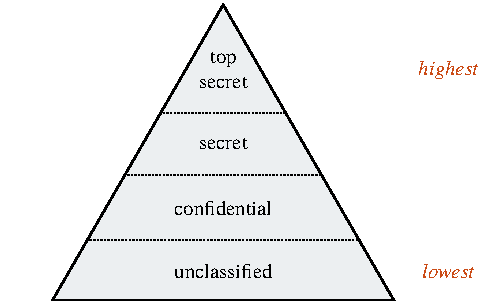
\includegraphics[]{fig_info-flow}
\caption[Document classification scheme]
{The United States federal government document classification scheme.}
\label{fig:us-docs}
\end{figure}


The main idea for achieving secure multilevel information flow is to impose constraints on how privileged information is permitted to flow within the system.
Secure information flow\index{information flow} is a confidentiality\index{confidentiality} guarantee, as it aims to ensure secrets do not leak\index{leak} to unauthorized parties~\cite{piessens2024}.
Implementing secure information flow requires three steps~\cite{eggert2014}.

\begin{enumerate} 

\item Identifying \emph{security classes}\index{security class} (alternatively, domains or user groups).
In~\autoref{fig:us-docs}, the classes are top secret, unclassified, secret, and confidential.

\item Defining a confidentiality \emph{policy}\index{information flow!policy}.
The policy specifies how information is permitted to flow between the security classes.
In~\autoref{fig:us-docs}, the the directed arrows define the policy.

\item Instrumenting an \emph{control}\index{information flow!control}. 
A control is a mechanism that enforces the behavior permitted by the policy.
In~\autoref{fig:us-docs}, no control is specified.

\end{enumerate}

For strong confidentiality\index{confidentiality} guarantees, the information flow approach should also consider and protect against side channels.
\emph{Side channels}\index{side channel} are all system characteristics that enable a malicious actor to deduce secrets,
indirectly and without assistance from other users~\cite[p. 280]{bishop2003}.
In terms of program executions, a few examples of side channels are termination, divergence, deadlocking, and execution latency.
 
\subsubsection{The Elements of Information Flow}
\label{if-elements}

\begin{description}

\item[Information flow]\index{information flow}
is an observable action between two agents\footnote{
The term \emph{agent} is to emphasize abstraction; an agent could be a human user, computer system, web request, program variable, \etc
} \({A}\) and \({B}\)~\cite{eggert2014}.
If an action performed by \({A}\) is observable to \({B}\),
then there exists an information flow from \({A}\) to \({B}\).
The information flow is \emph{explicit}\index{information flow!explicit} 
if it is directly observable from a single action.
The insecure program in~\autoref{lst:bool-ops} shows an example of direct information flow between \pr|high| and \pr|ret|.
Information flow is \emph{implicit}\index{information flow!implicit} 
when it is not directly observable, but the initial action can be deduced from the sequence of actions that follow.
The insecure program in~\autoref{lst:hi-cond} shows an example of an implicit flow.
The initial value of variable \pr|h| is deducible from the returned value \pr|l|, even though there is no direct flow from \pr|h| to \pr|l|.

\item[Information flow policy] (IFP)\index{information flow!policy}
is a statement of what is, and what is not, permissible between security classes~\cite[p. 9]{bishop2003}.
Since the seminal works on information flow~\cite{biba1977,bell1976}, it has been a convention to model information flow policies with lattices~\cite{denning76}\index{lattice}.
The most simple case considers two security classes, 
typically \enquote{high} and \enquote{low} \(({h}, {l})\) (or trusted and untrusted, secret and public, \etc).
In the simple case, the policy condition is that no information should flow from high to low.~\cite{bossi2005}
Then, showing that such a system is secure requires proving that executions that differ only on secrets are indistinguishable~\cite{piessens2024}.
% Transitive vs intransitive policies see, ~\cite{rushby1992}.
A policy that restricts information flow from a lower security class to a higher security class is called a
{non-interference policy}\index{non-interference}, presented in~\autoref{subsec:ni}.

\item[Information flow control] (IFC)\index{information flow!control}
is a mechanism that enforces a {policy\index{information flow!policy}}~\cite{bishop2003}.
Designing adequately expressive and effective controls is an active topic in security research~\cite{vandermeyden2007,bossi2005,sabelfeld2003}.
Like in static analysis (\cf~\autoref{static-analysis-basics}), designing a sound and complete control for arbitrary programs is impossible.
A sound IFC guarantees to find all policy violations\index{violation} and a precise IFC avoids raising excessive false alarms.
However, an overly restrictive IFC is challenging because it compromises availability\index{availability}.
The challenge of information flow control is more nuanced than classic data-flow analysis of functional properties,
because an IFC must consider a program \wrt policies and multiple executions~\cite{frumin2021}.
Thus, the same program can have multiple judgments depending on the policy.

\item[Declassification]\index{declassification}
refers to controlled release of secret information~\cite{sabelfeld2009}.
Declassification\index{declassification} requires a \emph{downgrading}\index{downgrading} operation;
a mechanisms that permits an elevated security judgement to be lowered.
In other words, information is allowed to flow contrary to the {policy\index{information flow!policy}}~\cite{cecchetti2017}.
Declassification\index{declassification} is necessary to support real world security applications.
For example, after a failed login attempt, an unauthorized user is able to observe the effect of the failure, 
although this is an information leak\index{leak}.
Declassification\index{declassification} is generally not safe~\cite{derakhshan2024}, 
and thus poses a major design challenge to IFCs\index{information flow!control}.
In the context of integrity\index{integrity}, declassification is also called {endorsement\index{endorsement}}~\cite{marion2011}.

\end{description}

\paragraph*{Secure and insecure information flows.}
Figures~\ref{lst:bool-ops}--\ref{lst:hi-cond} show basic examples of insecure and secure information flows\index{information flow}.
Variables \pr|high|, \pr|secret|, and \pr|h| are assumed to be secret and their values should not leak\index{leak} from executions.
The programs are fragments from the {IFSPEC benchmark suite}~\cite{hamann2018}\index{IFSPEC} available at~\cite{ifspec}.
The more advanced benchmarks involve, \eg aliasing, reflection, context sensitivity, and exception handling.

\begin{center}
\captionsetup{type=lstlisting}
\begin{minipage}{.45\textwidth}
\begin{center}\javainputlisting{bool-insecure.java}{Insecure.}\end{center}
\end{minipage}\hfill%
\begin{minipage}{.45\textwidth}
\begin{center}\javainputlisting{bool-secure.java}{Secure.}\end{center}
\end{minipage}
\captionof{lstlisting}[Secure and insecure Boolean operations]{
Boolean Operations. The programs are parametric on a Boolean variable \pr|high|.
In the insecure version, the value of \pr|high| is deducible from the value of \pr|ret|.
}\label{lst:bool-ops}
\end{center}

\begin{center}
\captionsetup{type=lstlisting}
\begin{minipage}{.45\textwidth}
\begin{center}\javainputlisting{array-insecure.java}{Insecure.}\end{center}
\end{minipage}\hfill%
\begin{minipage}{.45\textwidth}
\begin{center}\javainputlisting{array-secure.java}{Secure.}\end{center}
\end{minipage}
\captionof{lstlisting}[Implicit information flow leak in an array]{
Arrays Implicit Leak. The insecure program's output reveals if the value of \pr|secret| is or is not 42.
This leak\index{leak} is small, since it corresponds to 1 bit of information.
However, the secure version reveals nothing about the value of \pr|secret|.}
\label{lst:ni-arrays}
\end{center}

\begin{center}
\captionsetup{type=lstlisting}
\begin{minipage}{.45\textwidth}
\begin{center}\javainputlisting{loop-insecure.java}{Insecure.}\end{center}
\end{minipage}\hfill
\begin{minipage}{.45\textwidth}
\begin{center}\javainputlisting{loop-secure.java}{Secure.}\end{center}
\end{minipage}
\captionof{lstlisting}[High conditional incremental leak]{
High Conditional Incremental Leak.
Through the returned value \pr|l|, the insecure version reveals implicitly\index{information flow!implicit} the value of the secret variable \pr|h|.
Compared to~\autoref{lst:ni-arrays}, the program reveals every value of \pr|h|, so the leak\index{leak} here is more significant.
In the secure version, the value of \pr|h| cannot be deduced by the same reasoning.
However, the secure version is also potentially vulnerable through a side channel\index{side channel},
if the loop execution time is observable to an attacker\index{attacker (adversary)}.}
\label{lst:hi-cond}
\end{center}

\subsubsection{Techniques for Information Flow Modeling and Analysis}
\label{if-techniques}

Information flow\index{information flow} can be modeled in several distinct ways.
One way to categorize these approaches is by how they model systems;
\eg state-based automata, trace-based model\index{trace-based model}, and process algebras~\cite{vandermeyden2007}.
The presentation in this dissertation is only concerned with approaches based on programming languages.
The study of security through programming languages is called 
{\emph{language-based security}\index{language-based security}}~\cite{schneider2001,sabelfeld2003}.
The goal of {language-based security\index{language-based security}} is to use principles of programming languages---semantics, analysis, type systems, rewriting, \etc---to strengthen application security.
However, to offer a point of comparison, we introduce briefly trace-based information flow\index{information flow!trace-based}.
The language-based and trace-based approaches have very little in common~\cite[p. 235]{eggert2014}.

\paragraph*{Language-based information flow.}
Language based security formulates information flow constructs through programming languages.
Program logics and security type systems\index{security type system} are among the common techniques~\cite{frumin2021}.
A security type system aims to guarantee the {security policy\index{information flow!policy}} induced by its {lattice\index{lattice}}~\cite{marion2011}.
Each variable is assigned a {{security type}\index{security type}}, \ie a label that indicates its {security class\index{security class}}.
A satisfactorily secure program must pass a compile-time type check of the security labels.
%Language-based information flow typically handles only the two-level security class hierarchy, 
%and does not address intransitive policies~\cite{vonoheimb2004}.
Sections~\ref{subsec:ni} and ~\ref{sec:anytime} discuss the {language-based\index{language-based security}} information flow in more detail.

\paragraph*{Trace-based information flow.}\index{information flow!trace-based}
The trace-based approach~\cite[p. 24]{eggert2014} models a system with a state machine.
In response to actions, the machine transitions, deterministically or nondeterministically\index{nondeterminism}, from state to state.
A \emph{trace}\index{trace} is a sequence of actions of such a machine~\cite{nelson2020}.
Evaluating secure information flow\index{information flow} over traces is about equivalence relations\index{equivalence relation}, 
or {indistinguishability}\index{indistinguishability}.
For example, for a policy\index{information flow!policy} that requires that secrets should not leak\index{leak} to public, 
two traces must be indistinguishable\index{indistinguishability} from the perspective of a public class (they only differ on secret actions).
Further, executing those traces should produce publicly indistinguishable\index{indistinguishability} final states~\cite{nelson2020}.
Showing that a trace-based system satisfies this security requirements is done by {simulation\index{simulation}}~\cite{piessens2024} 
where the simulation proves the trace equivalence \wrt a policy.

\paragraph*{Formal security analysis.}\index{security analysis}
Establishing that a \enquote{system is secure} demands security analysis.
Rigorous formal security analysis considers the following three aspects.

\begin{enumerate}

\item \emph{System model}\index{system model}: a precise mathematical definition of the system to be secured.

\item \emph{Security objective}\index{security objective} (or properties\index{security property}): 
a specification of system behaviors that are considered secure.

\item \emph{Attack model\index{attack model}} (or threat model\index{threat model}): 
a definition of the class of attacks against which the system should be secure.

\end{enumerate}
The parenthesized terms are included because the literature~\cite{bognar2022, bau2011} varies in exact terminology.
However, the goal of formal security analysis\index{security analysis} is uniform.
For a satisfactory system, a formal analysis must conclude with a proof that shows the system satisfies its security specification under the identified threat.
Designing an adequate system model\index{system model}, 
security objective\index{security objective}, 
and attack model\index{attack model} to formally prove system security is nontrivial~\cite{piessens2024}.

\subsubsection{A Primer on Non-Interference}
\label{subsec:ni}

Non-interference\index{non-interference}
is a foundational family of security policies\index{information flow!policy} and security properties\index{security property}
 that constrains information flow\index{information flow} during computations.
The important idea is that a low(er) security class is not permitted to observe a high(er) security class.
In other words, information flow from high to low security class is not allowed.
%Establishing that a system is non-interfering requires showing that behavior of high security class has no impact on low security class.
%(alternatively, that the low level view is independent of the high level).
Although non-interference\index{non-interference}
 is often described in binary terms, referring to just two security classes\index{security class}, it is applicable to arbitrary security hierarchies\footnote{The policy in \autoref{fig:us-docs} is a 4-class non-interference policy.}.
The primary application of non-interference\index{non-interference} 
is in supporting multilevel security\index{multilevel security} systems~\cite{roscoe1999}.

\paragraph*{Classic non-interference.}
The concept of \emph{non-interference}\index{non-interference} was introduced in 1982 by Joseph Goguen and José Meseguer.
Their seminal paper~\cite{goguen1982} presented the concept (only) informally, as follows.
\begin{quotation}
\noindent One group of users, using a certain set of commands, is non-interfering with another group of users if what the first group does with those commands has no effect on what the second group of users can see.
\end{quotation}
Broadly, the paper provided an early framework for formal modeling and verification of information flow\index{information flow}
over deterministic state machines.
This early view of deterministic non-interference\index{non-interference} is regarded as \emph{classical non-interference}~\cite{focardi1997}.

The terminology around non-interference\index{non-interference} and confidentiality\index{confidentiality} 
is somewhat inconsistent~\cite{sabelfeld2003,vandermeyden2007}.
For example, surveying mathematical formalizations, Nelson et al.~\cite{nelson2020} 
identified four distinct characterizations of non-interference\index{non-interference}.
It therefore more accurate to consider non-interference\index{non-interference} as a family of 
information flow\index{information flow} properties that share the above common core.
Non-interference\index{non-interference} has been studied in in a variety of models, 
\eg \ndx{trace-based model}s,
process calculi, programming languages, probabilistic models, timed models, and {cryptographic protocols\index{cryptography}}~\cite{bossi2005}.
\autoref{sec-types} will present how to formulate non-interference in terms of programming languages.

\paragraph*{Practical challenges with non-interference.}
Non-interference is a strong notion because it includes the absence of both 
explicit\index{information flow!explicit} and implicit\index{information flow!implicit} information flows~\cite{bossi2005}.
As noted by many authors~\cite{cecchetti2017,bossi2005}, the requirement is too strong for practical applications.
Strict non-interference is not achievable in real world systems~\cite{bossi2005}.
The non-interference requirement may also be excessively restrictive when additional knowledge about the system is available~\cite{bossi2005}.
For example, consider two \enquote{high} users communicating over an encrypted channel,
 and a \enquote{low} user who can observe the communication events.
In this case, there is an implicit\index{information flow!implicit} flow about the event, but the exchanged information remains secret.
Such controlled leak may be practically acceptable, but classic non-interference would not permit it.
Declassification\index{declassification} (\cf~\autoref{if-security}) allows controlled and restricted 
information flows\index{information flow} against the non-interference policy\index{information flow!policy}.
It is an important mechanism to support security requirements of real world systems.

Proving that a system satisfies non-interference is harder than proving functional correctness~\cite{frumin2021}.
The reason is that functional correctness is a property of each single program execution.
Non-interference, when expressed with trace-based information flow, is stated over multiple runs of the same program.
A non-interference proof requires showing that for different behaviors of high security class the low security class cannot observe any different behavior~\cite{frumin2021}.
When a program property is expressed over a set of trace properties it is called a {\emph{hyperproperty}\index{hyperproperty}}~\cite{clarkson2010}.
Since a non-interference\index{non-interference} proof requires sets of execution traces, 
{non-interference\index{non-interference}} is a {hyperproperty\index{hyperproperty}}~\cite{mastroeni2019}.

\paragraph*{Extensions.}
The classic definition of {non-interference\index{non-interference}} has been extended in several directions.
The following list contains several variants, though the list is necessarily incomplete.
See~\cite{vandermeyden2010,nelson2020,eggert2014} for comprehensive expositions of {non-interference\index{non-interference}} comparisons of the different varieties.
{Progress-sensitive non-interference\index{non-interference!progress-sensitive}} is consider the gold standard of non-interference based information flow\index{information flow} security~\cite{derakhshan2024}.

\begin{itemize}

\item\emph{Bipartite non-interference}~\cite{aceto2024}\index{non-interference!bipartite}
is defined in terms of two levels, low and high.

\item\emph{Nondeterministic non-interference} (NNI)~\cite{focardi1997}\index{non-interference!nondeterministic}
is a generalization of classic non-interference to nondeterministic systems.

\item\emph{Termination-Insensitive noninterference} (TINI)~\cite{hedin2012}\index{non-interference!termination-insensitive}
requires that terminating executions satisfy non-interference.

\item\emph{Termination-sensitive noninterference} (TSNI)~\cite{hedin2012}\index{non-interference!termination-sensitive}
extends classic non-interference by considering divergence as distinguishable from termination,
requiring that the behavior must be consistent for all executions.

\item\emph{Progress insensitive non-interference} (PINI)~\cite{bay2020}\index{non-interference!progress-insensitive}
generalizes termination-insensitive non-interference to accommodate I/O interactions,
where executions agree stepwise on same observable behaviors, permitting silent divergence.

\item\emph{Progress sensitive non-interference} (PSNI)~\cite{hedin2012}\index{non-interference!progress-sensitive}
demands that executions agree on making stepwise progress and match on the public observables.

\item\emph{Deadlock-sensitive non-interference} (DSNI)~\cite{vandenheuvel2024}\index{non-interference!deadlock-sensitive}
considers deadlocking as an observable behavior,
and requires executions agree on deadlocking behavior.

\item\emph{Intransitive non-interference}~\cite{roscoe1999}\index{non-interference!intransitive}
is a relaxed notion of non-interference, where implicit flows may be permitted.

\end{itemize}
Finally, a note on \emph{non-leakage}\index{non-leakage} and \emph{non-influence}\index{non-influence}~\cite{vonoheimb2004}.
The terms recur in information flow\index{information flow} literature, \eg~\cite{nelson2020,ileri2024};
and are related to {non-interference\index{non-interference}}, but different.
While non-interference restricts information flow \emph{between} security classes,
{{non-leakage}\index{non-leakage}} is a view-partitioning constraint --
it restricts the \emph{parts of system state} a security class is allowed to infer.
Non-leakage considers the same trace\index{trace} over two states (instead of two traces over same states).
The expectation is that executing the same trace from the two states should result in indistinguishable states~\cite{nelson2020}.
Finally, {{non-influence}\index{non-influence}} is the combination of non-interference (as defined in~\cite{rushby1992}) and non-leakage.

\subsubsection{Non-Interference With Security Types}
\label{sec-types}

In the context of programming languages, a program is {non-interfering\index{non-interference}} if 
{secret (high) inputs} do not affect the calculation of {public (low) outputs}~\cite{sabelfeld2003}.
The idea to use programming languages to model {non-interference\index{non-interference}} was introduced by~\textcite{volpanoI1996}.
The paper shows that {non-interference\index{non-interference}} can be soundly approximated using a {security type system\index{security type system}}.
The influential result has since then been followed by numerous works in language-based security.
Among a few examples, {non-interference\index{non-interference}} has been studied in terms of
static program analysis~\cite{barthe2007,huang2014},
{secure compilation\index{secure compilation}}~\cite{patrignani2017,myers1999,cecchetti2017},
formal methods~\cite{kammuller2008,nelson2020},
program logics~\cite{frumin2021,karbyshev2018,garg2006,beringer2007},
verification~\cite{eilers2023},
and \ndx{software testing}~\cite{hritcu2013}.
In general, evaluating {non-interference\index{non-interference}} over at different levels of abstractions
(compilation, instruction set architecture, processor, hardware, digital circuits) is necessary,
because even if a program is {non-interfering\index{non-interference}} \wrt its syntax,
it is not protected against vulnerabilities occurring at lower abstraction levels~\cite{piessens2024}.
To develop intuition of programming languages based {non-interference\index{non-interference}},
the rest of this subsection shows examples using {a security type system\index{security type system}} adapted from~\cite{sabelfeld2003}\footnote{
The system is equivalent to Volpano et al. but more conventional in style.}.

\paragraph*{Programs, non-interference, and typing rules.}
For a programming language, we consider the grammar\index{grammar} shown in ~\autoref{fig:ni-syntax}.
A program (command) in this language is denoted by \pr|C|.
Computation starts in an input state with high and low variables \(s = (s_h, s_l)\).
Either \pr|C| terminates in an output state with final values \(s' = (s_h', s_l')\), or diverges, which we denote by \(\bot\).
Letting \(S\) be the set of input states, \(s \in S \),
%The semantics \(\sem{\text{\pr|C|}}\) map an input state \(s \in S \) either to an output state \(\sem{\text{\pr|C|}}s \in S\) or to divergence.
the semantics \(\sem{\text{\pr|C|}}\) of \pr|C| is defined by a function \(\sem{\text{\pr|C|}} : S \rightarrow S_\bot \) where \( S_\bot = S \cup \{ \bot \} \) and \( \bot \notin S\).
The variation of high input is an equivalence relation\index{equivalence relation} \(=_L\).
Two inputs are equivalent if they agree on low values, \ie \(s =_L s'\) iff \( s_l = s_l' \).
The attacker's\index{attacker (adversary)} observational power is characterized by a relation on behaviors defined by the semantics, denoted \(\approx_L\).
Two behaviors are related by \(\approx_L\) iff they are indistinguishable\index{indistinguishability} to the attacker\index{attacker (adversary)}.
%The relation \(\approx_L\) reflects the low security class viewpoint of the system.
Formally, program \pr|C| is secure \wrt non-interference iff
\begin{align*}
\forall s_1,s_2, \in S \cdot s_1 =_L s_2 \implies \sem{C}_{s_1} \approx_L \sem{C}_{s_2}
\end{align*}
which reads:
\begin{quotation}
\noindent If two input states share the same low values, then the behaviors of the program executed on these states are indistinguishable by the attacker\index{attacker (adversary)}.
\end{quotation}
The security typing rules are shown in~\autoref{fig:ni-types}.
For the typing rules, an expression \(\vdash\prm{e} : \tau\) means \pr|e| has type \(\tau\).
The judgement \(\Gamma\vdash\text{\pr|C|}\) means the program \pr|C| is typable in security context \({\Gamma}\).
Expression types and security contexts can be either low (\({l}\)) or high (\({h}\)).
The symbol \(\Gamma\) refers to the current context (low or high).

\begin{figure}[t]
\centering\begin{align*}
C \, ::={ }& \, \mathbf{skip} \mid
\mathbf{v}\coloneqq{}\mathbf{e} \mid
\nonterm C_{{\mathrm{1}}}  \ottsym{;}  \nonterm C_{{\mathrm{2}}} \mid
\ottkw{if} \, \ottkw{e} \, \ottkw{then} \, \nonterm C_{{\mathrm{1}}} \, \ottkw{else} \, \nonterm C_{{\mathrm{2}}} \mid
\ottkw{while} \, \ottkw{e} \, \ottkw{do} \, \nonterm C
\end{align*}
\caption[Grammar of the non-interference security type system]
{Grammar of the non-interference security type system.}\label{fig:ni-syntax}
\end{figure}
\begin{figure}[t]
\centering\drules[E]{$\vdash \prm{e} : \tau$}{expression typing}{High,Low}
\centering\drules[C]{$\Gamma \vdash \text{\pr|C|}$}{command typing}{Skip,AssignOne,AssignTwo,Seq,While,If,Sub}
\caption[Non-interference security type system]{A non-interference security type system.}\label{fig:ni-types}
\end{figure}

\paragraph*{Derivations.}
Consider the programs in Figures~\ref{lst:bool-ops}--\ref{lst:hi-cond}.
Since the programs are written in Java\index{Java}, the constructs are richer than available in the type system grammar\index{grammar}.
The programs are not fully analyzable.
For example, the {security type system\index{security type system}} does not specify how to handle the array in~\autoref{lst:ni-arrays}.
However, we can analyze sub-programs, like the \pr|while| loops in~\autoref{lst:hi-cond} through a mapping to the grammar.
The following examples show basic non-interference\index{non-interference} derivations.

\begin{example}[Secure high conditional incremental leak]\label{ex:high-cond-sec}
We will analyze the following program fragment.

\begin{center}
\begin{minipage}{\textwidth}
\javainputlisting[][linerange={2-2},numbers=none]{loop-secure.java}
\end{minipage}
\end{center}

We assume \pr|h| is an arbitrarily typed variable---neither low or high---and will analyze both cases.
We map the program to the grammar by substituting \pr|h > 0| with \pr|e|₀ and \pr|h--| with \pr|v:=e|₁\footnote{
We lose detail of the compound assignment, but the loss is acceptable for this example.}
to obtain \pr|while(e$_0$) { v:=e$_1$ }|.

\paragraph*{Case 1:  \pr|e|₀, \pr|v|, and \pr|e|₁ are of type high.}
Since the program is derivable as follows, it is non-interfering.

\begin{center}\begin{prooftree}
\infer0[\textsc{E-High}]{\vdash \prm{e}₀ : \mathbf{h}}
\infer0[\textsc{C-Assign1}]{\mathbf{h} \vdash \prm{v:=e}₁}
\infer2[\textsc{C-While}]{\mathbf{h} \vdash \prm{while(e$_0$) \{ v:=e$_1$ \}}}
\end{prooftree}\end{center}

\paragraph*{Case 2: \pr|e$_0$|, \pr|v|, and \pr|e$_1$| are of type low.}
The program is also derivable in low context, and again, is non-interfering.

\begin{center}\begin{prooftree}
\hypo{\mathbf{h} \notin \text{vars}(\prm{e}₀)}
\infer1[\textsc{E-Low}]{\vdash \prm{e}₀ : \mathbf{l}}
\hypo{\mathbf{h} \notin \text{vars}(\prm{v:=e}₁)}
\infer1[\textsc{E-Low}]{\vdash \prm{v:=e}₁ : \mathbf{l}}
\infer1[\textsc{C-Assign2}]{\mathbf{l} \vdash \prm{v:=e}₁}
\infer2[\textsc{C-While}]{\mathbf{l} \vdash \prm{while(e$_0$) \{ v:=e$_1$ \}}}
\end{prooftree}\end{center}

Intuitively, the program is always non-interfering because it processes only high (secret) values, or low (public) values;
never mixing the two security classes.
\end{example}

\begin{example}[Insecure high conditional incremental leak]\label{ex:high-cond-insecure}
We analyze the following program.
It is labeled insecure in the benchmark suite.

\begin{center}
\begin{minipage}{\textwidth}
\javainputlisting[][linerange={2-2},numbers=none]{loop-insecure.java}
\end{minipage}
\end{center}

The goal of this example is to reveal the \ndx{assumption}s that make it insecure.
Using a similar procedure as in~\autoref{ex:high-cond-sec}, we express the program in the type system grammar as
\begin{center}
\pr|while(e$_0$) { v$_1$:=e$_1$; v$_2$:=e$_2$ }|
\end{center}
To maintain the original information flow\index{information flow} behavior,
expressions  \pr|e|₀, \pr|v|₁,  \pr|e|₁
(\resp \pr|v|₂ and \pr|e|₂) must be typable in the same security class\index{security class}.
We also know from \autoref{ex:high-cond-sec} that without multiple security classes\index{security class},
the program is non-interfering\index{non-interference}.
There are two interesting cases.

\paragraph*{Case 1: \pr|e|₀, \pr|v|₁, \pr|e|₁ are high, and \pr|v|₂, \pr|e|₂ are low.}
The derivation beings as follows.

\begin{center}\begin{prooftree}
\infer0[\textsc{E-High}]{\vdash \prm{e}₀ : \mathbf{h}}
\infer0[\textsc{C-Assign1}]{\mathbf{h} \vdash \prm{v}₁\prm{:=e}₁}
\infer0[]{\text{\circled[red]{\normalfont{\textbf{\texttt{X}}}}} \vdash \prm{v}₂\prm{:=e}₂}
\infer2[\textsc{C-Seq}]{\mathbf{h} \vdash \prm{v$_1$:=e$_1$; v$_2$:=e$_2$}}
\infer2[\textsc{C-While}]{\mathbf{h} \vdash \prm{while(e$_0$) \{ v$_1$:=e$_1$; v$_2$:=e$_2$ \}}}
\end{prooftree}\end{center}

Since \pr|v|₂ is of type low, there is no way to handle \pr|v|₂\pr|:=e|₂.
The derivation gets stuck at point marked{ }{ }{\circled[red]{\textbf{\texttt{X}}}}{ }because the program has a non-interference\index{non-interference} violation.
Intuitively, it is because the program operates on a low variable inside a loop with a guard variable\index{guard variable} that is of type high.
This construction is not safe because it leaks information.

\paragraph*{Case: \pr|e|₀, \pr|v|₁, \pr|e|₁ are low and \pr|v|₂, \pr|e|₂ are of type high.}

\begin{center}\begin{prooftree}
\hypo{\mathbf{h} \notin \text{vars}(\prm{e}₀)}
\infer1[\textsc{E-Low}]{\vdash \prm{e}₀ : \mathbf{l}}
\hypo{\mathbf{h} \notin \text{vars}(\prm{e}₁)}
\infer1[\textsc{E-Low}]{\vdash \prm{e}₁ : \mathbf{l}}
\infer1[\textsc{C-Assign2}]{\mathbf{l} \vdash \prm{v}₁\prm{:=e}₁}
\infer0[\textsc{C-Assign1}]{\mathsf{h} \vdash \prm{v}₂\prm{:=e}₂}
\infer1[\textsc{C-Sub}]{\mathsf{l} \vdash \prm{v}₂\prm{:=e}₂}
\infer2[\textsc{C-Seq}]{\mathbf{l} \vdash
\prm{v}_\prm{1}\prm{:=e}_\prm{1}\prm{;}\prm{v}₂\prm{:=e}₂}
\infer2[\textsc{C-While}]{\mathbf{l} \vdash\prm{while(e$_0$) \{ v$_1$:=e$_1$; v$_2$:=e$_2$ \}}}
\end{prooftree}\end{center}

Reversing the security label configuration makes the program typable.
A critical rule is \textsc{C-Sub} (subsumption) that permits lowering the security class label of a high command.
Unlike in the previous case, the loop guard\index{guard variable} is now low type.
It permits manipulating a variable of high type inside the loop body.
\end{example}

\subsubsection{Security Meets Implicit Computational Complexity}
\label{icc-sec}

With a common focus on restrictions, it seems intuitive that 
techniques from implicit computational complexity would pair elegantly with information flow and applications in \ndx{language-based security}.
The combination can potentially provide two types of correctness guarantees, relating resource analysis and security.
Supporting this hypothesis, there are already multiple series of work exploring connections between the two domains.
This section gives a brief summary of those results.

\paragraph*{Complexity via non-interference: SAFE programs.}
The class of \ndx{SAFE programs} is foundational in demonstrating that non-interference \ndx{security type system}s can support implicit characterizations of \ndx{complexity classes}.
The idea was introduced by Jean-Yves Marion in~\cite{marion2011}.
\ndx{SAFE programs} continue to be actively investigated by Marion, Emmanuel Hainry, Romain Péchoux, and others.

Starting with the principle of {\emph{\ndx{tiering}}}\footnote{
The intuition behind tiering, \aka \ndx{ramification}, is that program execution time depends on the nature of information flow during executions.
The flow can be constrained by imposing a precedence relation that regulates the information flow,
\eg from higher tier to lower tier~\cite{leivant1995, leivant2013}.},
Marion extended the principle to characterize the class of polynomial time computable functions\ccxi{p}.
A critical step in obtaining this result was combining tiering with a type system\index{security type system} for secure \ndx{information flow}.
Each variable is assigned a type -- a {tier} of either 0 or 1 -- representing elements of a complexity \ndx{lattice}.
The paper then shows that terminating and well-typed programs are computable in polynomial time.
\ndx{SAFE programs} is precisely the class of programs captured by this characterization.

Judging by the number of works that followed, the technique was inspirational.
The subsequent results have provided extensions mainly along two directions.
The first has focused on programming language paradigms, including: 
concurrent fork-join processes (\ndx{SAFE processes})~\cite{hainry2013},
dynamic data structure (ramified programs)\index{ramified programs}~\cite{leivant2013}, and
{object-oriented (OO) programs\index{SAFE programs!object-oriented}}~\cite{hainry2015}.
The OOP result is the first characterization of polynomial time\ccxi{p} computable functions in the object oriented paradigm.
The second directions has focused on redefining the system restrictions, with the goal of improving intensional \ndx{completeness}.
For example, the class of stratified programs\index{stratified programs}~\cite{hainry2023} characterizes a strictly larger class than SAFE programs,
by using a combination of {security type system\index{security type system}}, heap memory restriction, and shape analysis\index{shape analysis}.
With the same end-goal, aperiodic programs (AP)~\cite{hainry2024}\index{aperiodic programs} extends SAFE programs by using declassification\index{declassification};
another mechanism adopted from the security domain.
In the latter, the main result is a proof that SAFE and terminating aperiodic programs is the class of Basic Feasible Functionals\index{Basic Feasible Functionals}, \ie \(\sem{\text{SAFE}\;\cap\;\text{AP}\;\cap\;\text{terminating} = \text{BFF}}\)~\cite{hainry2020,hainry2024}.

\paragraph*{From complexity to \ndx{cryptography}.}
A separate series of works applies implicit computation complexity toward applications in \ndx{cryptography}.
The application is natural, because the security of cryptographic\index{cryptography} schemes is formulated as a mathematical problem, where the goal is to show the scheme is not to be solvable by a feasible adversary.
The term feasible refers to computable in polynomial time~\cite{feree2018}.

This application is naturally, because in showing that a cryptographic\index{cryptography} scheme is secure, adversarial capabilities must restrict available computational power~\cite{heraud2011}.

\begin{description}

\item[formalized safe recursion.]
The formalization of \ndx{safe recursion} (\cf~\autoref{safe-rec}) was primarily motivated by its envisioned usefulness in \ndx{cryptography}~\cite{heraud2011}. At the time, the method was integrated into \href{https://github.com/EasyCrypt/certicrypt}{CertiCrypt} framework (predecessor of \ndx{EasyCrypt}), to provide complexity guarantees.
However, proofs of complexity bounds are

\item[Type system d\(\ell\)T.]
The type system \ndx{d\(\ell\)T}~\cite{baillot2015,baillot2019} is simultaneously complexity-aware and has capabilities to support cryptographic proofs\index{cryptography}.
Among its applications, d\(\ell\)T allows proving that the constructed adversary for the \ndx{Goldreich-Levin theorem} is polynomial time\ccxi{p}.
Such applications are interesting because they involve computations that are inherently non-polynomial in \ndx{time complexity}.
Thus, handling such sub-computations requires pushing ICC techniques beyond their usual capabilities.
A limitation of the type system is that it has not been implemented.

\end{description}
Both \ndx{d\(\ell\)T} and the formalization of \ndx{safe recursion} have inspired other mechanized proofs~\cite{barbosa2021,feree2018}.

\subsubsection{From Quasi-Invariant Chunks to Non-Interference}
\label{subsubsec:quasi-ni}

Reinforcing the existing connections,~\autoref{sec:anytime} presents a program logic for \ndx{non-interference}.
The logic is inspired by implicit computational complexity.
The motivating idea was to explore the power and utility of ICC techniques in \ndx{language-based security} analysis.

The logic analyzes \ndx{information flow}s in \ndx{imperative programs}.
It abstracts information flow patterns between variables into matrices.
Once the matrix is paired with a security policy, it is possible to evaluate whether the program satisfies an \emph{anytime non-interference} property, which is introduced in the paper.

The technique is a refinement of prior works (refer to~\autoref{sec:vmcai} and~\cite{moyen20172}).\footnote{
For ease and consistency, we dub the technique (informally) as the \emph{QI framework}.}
A previous version of the logic was used to obtain a compile-time program optimization.
Although the logic no longer guarantees complexity bounds, it demonstrates the utility of interchanging techniques between the ICC and security.

Adjusting the logic to track \ndx{non-interference} revealed various mathematical insights.
For example, the treatment of loops is more straightforward for \ndx{non-interference} than in \ndx{complexity analysis},
because the former requires no fixed point computations.
As a \ndx{data flow analysis}, that tracks different program properties based on \emph{dependence},
the technique is reminiscent of the \ndx{Dependency Core Calculus} (DCC)~\cite{abadi1999b}.
The multiplicity of the program logic suggests it may possess representational capabilities similar to DCC\@.
